\protect\hyperlink{main-nav}{≡} \protect\hyperlink{close-nav}{×}

\hypertarget{section-2.10-other-applications}{%
\section{Section 2.10: Other
Applications}\label{section-2.10-other-applications}}

\hypertarget{tangent-line-approximation}{%
\subsection{Tangent Line
Approximation}\label{tangent-line-approximation}}

Back when we first thought about the derivative, we used the slope of
secant lines over tiny intervals to approximate the derivative:
\textbackslash{}{[} f'(a)\textbackslash{}approx
\textbackslash{}frac\{\textbackslash{}Delta y\}\{\textbackslash{}Delta
x\}=\textbackslash{}frac\{f(x)-f(a)\}\{x-a\}\textbackslash{}{]}

Now that we have other ways to find derivatives, we can exploit this
approximation to go the other way. Solve the expression above for
\textbackslash{}(f(x)\textbackslash{}), and you'll get the tangent line
approximation:

\hypertarget{the-tangent-line-approximation-tla-or-linear-approximation}{%
\paragraph{The Tangent Line Approximation (TLA) (or ``Linear
Approximation'')}\label{the-tangent-line-approximation-tla-or-linear-approximation}}

To approximate the value of \textbackslash{}(f(x)\textbackslash{}) using
TLA, find some \textbackslash{}(a\textbackslash{}) where

\begin{enumerate}
\tightlist
\item
  \textbackslash{}(a\textbackslash{}) and
  \textbackslash{}(x\textbackslash{}) are ``close,'' and
\item
  You know the exact values of both
  \textbackslash{}(f(a)\textbackslash{}) and
  \textbackslash{}(f'(a)\textbackslash{}).
\end{enumerate}

Then \textbackslash{}{[}f(x) \textbackslash{}approx
f(a)+f'(a)(x-a).\textbackslash{}{]}

Another way to look at the same formula:
\textbackslash{}{[}\textbackslash{}Delta y\textbackslash{}approx
f'(a)\textbackslash{}Delta x\textbackslash{}{]}

How close is close? It depends on the shape of the graph of
\textbackslash{}(f\textbackslash{}). In general, the closer the better.

\begin{figure}
\centering
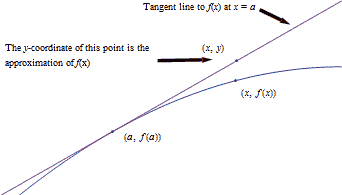
\includegraphics{images/image099.png}
\caption{}
\end{figure}

To view this video please enable JavaScript, and consider upgrading to a
web browser that \href{http://videojs.com/html5-video-support/}{supports
HTML5 video}

Try it for yourself using this applet (click the button next to L(x) if
the line isn't showing up):

\hypertarget{applet_container}{}

\hypertarget{example-1}{%
\paragraph{Example 1}\label{example-1}}

Suppose we know that \textbackslash{}(g(20) = 5\textbackslash{}) and
\textbackslash{}(g'(20) = 1.4\textbackslash{}). Use this information to
approximate \textbackslash{}(g(23)\textbackslash{}) and
\textbackslash{}(g(18)\textbackslash{}).

Using the tangent line approximation: \textbackslash{}{[}
\textbackslash{}begin\{align*\} g(23)\textbackslash{}approx \& 5 +
(1.4)(23 - 20) = 9.2\textbackslash{}\textbackslash{}
g(18)\textbackslash{}approx \& 5 + (1.4)(18 - 20) = 2.2
\textbackslash{}end\{align*\} \textbackslash{}{]}

Note that we don't know if these approximations are close -- but they're
the best we can do with the limited information we have to start with.
Note also that 18 and 23 are sort of close to 20, so we can hope these
approximations are pretty good. We would feel more confident using this
information to approximate \textbackslash{}(g(20.003)\textbackslash{}).
We would feel very unsure using this information to approximate
\textbackslash{}(g(55)\textbackslash{}).

\hypertarget{elasticity}{%
\subsection{Elasticity}\label{elasticity}}

We know that demand functions are decreasing, so when the price
increases, the quantity demanded goes down. But what about revenue =
price \textbackslash{}( \textbackslash{}times \textbackslash{})
quantity? When the price increases will revenue go down because the
demand dropped so much? Or will revenue increase because demand didn't
drop very much?

Elasticity of demand is a measure of how demand reacts to price changes.
It's normalized -- that means the particular prices and quantities don't
matter, and everything is treated as a percent change. The formula for
elasticity of demand involves a derivative, which is why we're
discussing it here.

\hypertarget{elasticity-of-demand}{%
\paragraph{Elasticity of Demand}\label{elasticity-of-demand}}

Given a demand function that gives \textbackslash{}(q\textbackslash{})
in terms of \textbackslash{}(p\textbackslash{}), the \textbf{elasticity
of demand} is
\textbackslash{}{[}E=\textbackslash{}left\textbar{}\textbackslash{}frac\{p\}\{q\}\textbackslash{}cdot
\textbackslash{}frac\{dq\}\{dp\}\textbackslash{}right\textbar{}\textbackslash{}{]}

(Note that since demand is a decreasing function of
\textbackslash{}(p\textbackslash{}), the derivative is negative. That's
why we have the absolute values -- so
\textbackslash{}(E\textbackslash{}) will always be positive.)

\begin{itemize}
\tightlist
\item
  If \textbackslash{}(E \textbackslash{}lt 1\textbackslash{}), we say
  demand is inelastic. In this case, raising prices increases revenue.
\item
  If \textbackslash{}(E \textbackslash{}gt 1\textbackslash{}), we say
  demand is elastic. In this case, raising prices decreases revenue.
\item
  If \textbackslash{}(E = 1\textbackslash{}), we say demand is unitary.
  \textbackslash{}(E = 1\textbackslash{}) at critical points of the
  revenue function.
\end{itemize}

\hypertarget{interpretation-of-elasticity}{%
\subsubsection{Interpretation of
elasticity}\label{interpretation-of-elasticity}}

If the price increases by 1\%, the demand will decrease by E\%.

\hypertarget{example-2}{%
\paragraph{Example 2}\label{example-2}}

A company sells \textbackslash{}( q \textbackslash{}) ribbon winders per
year at \$\textbackslash{}( p \textbackslash{}) per ribbon winder. The
demand function for ribbon winders is given by \textbackslash{}(
p=300-0.02q \textbackslash{}). Find the elasticity of demand when the
price is \$70 apiece. Will an increase in price lead to an increase in
revenue?

First, we need to solve the demand equation so it gives
\textbackslash{}( q \textbackslash{}) in terms of \textbackslash{}( p
\textbackslash{}), so that we can find \textbackslash{}(
\textbackslash{}frac\{dq\}\{dp\} \textbackslash{}): \textbackslash{}(
p=300-0.02q \textbackslash{}), so \textbackslash{}( q=15000-50p
\textbackslash{}). Then \textbackslash{}(
\textbackslash{}frac\{dq\}\{dp\}=-50 \textbackslash{}).

We need to find \textbackslash{}( q \textbackslash{}) when
\textbackslash{}( p = 70 \textbackslash{}): \textbackslash{}{[} q =
11500. \textbackslash{}{]}

Now compute \textbackslash{}{[} E=\textbackslash{}left\textbar{}
\textbackslash{}frac\{p\}\{q\}\textbackslash{}cdot\textbackslash{}frac\{dq\}\{dp\}
\textbackslash{}right\textbar{}=\textbackslash{}left\textbar{}
\textbackslash{}frac\{70\}\{11500\}\textbackslash{}cdot(-50)
\textbackslash{}right\textbar{} \textbackslash{}approx 0.3
\textbackslash{}{]}

\textbackslash{}(E \textbackslash{}lt 1\textbackslash{}), so demand is
inelastic. Increasing the price by 1\% would only cause a 0.3\% drop in
demand. Increasing the price would lead to an increase in revenue, so it
seems that the company should increase its price.

The demand for products that people have to buy, such as onions, tends
to be inelastic. Even if the price goes up, people still have to buy
about the same amount of onions, and revenue will not go down. The
demand for products that people can do without, or put off buying, such
as cars, tends to be elastic. If the price goes up, people will just not
buy cars right now, and revenue will drop.

To view this video please enable JavaScript, and consider upgrading to a
web browser that \href{http://videojs.com/html5-video-support/}{supports
HTML5 video}

\hypertarget{example-3}{%
\paragraph{Example 3}\label{example-3}}

A company finds the demand \textbackslash{}( q \textbackslash{}), in
thousands, for their kites to be \textbackslash{}( q=400-p\^{}2
\textbackslash{}) at a price of \textbackslash{}( p \textbackslash{})
dollars. Find the elasticity of demand when the price is \$5 and when
the price is \$15. Then find the price that will maximize revenue.

Calculating the derivative, \textbackslash{}(
\textbackslash{}frac\{dq\}\{dp\}=-2p \textbackslash{}). The elasticity
equation as a function of \textbackslash{}( p \textbackslash{}) will be:
\textbackslash{}{[} E=\textbackslash{}left\textbar{}
\textbackslash{}frac\{p\}\{q\}\textbackslash{}cdot\textbackslash{}frac\{dq\}\{dp\}
\textbackslash{}right\textbar{}=\textbackslash{}left\textbar{}
\textbackslash{}frac\{p\}\{400-p\^{}2\}\textbackslash{}cdot (-2p)
\textbackslash{}right\textbar{} =\textbackslash{}left\textbar{}
\textbackslash{}frac\{-2p\^{}2\}\{400-p\^{}2\}
\textbackslash{}right\textbar{} \textbackslash{}{]}

Evaluating this to find the elasticity at \$5 and at \$15:

\textbackslash{}{[} E = \textbackslash{}left\textbar{}
\textbackslash{}frac\{-2(5)\^{}2\}\{400-(5)\^{}2\}
\textbackslash{}right\textbar{} \textbackslash{}approx 0.133
\textbackslash{}{]} So the demand is inelastic when the price is \$5.

At a price of \$5, a 1\% increase in price would decrease demand by only
0.133\%. Revenue could be raised by increasing prices.

\textbackslash{}{[} E = \textbackslash{}left\textbar{}
\textbackslash{}frac\{-2(15)\^{}2\}\{400-(15)\^{}2\}
\textbackslash{}right\textbar{} \textbackslash{}approx 2.571
\textbackslash{}{]} So the demand is elastic when the price is \$15.

At a price of \$15, a 1\% increase in price would decrease demand by
2.571\%. Revenue could be raised by decreasing prices.

To maximize the revenue, we could solve for when \textbackslash{}( E = 1
\textbackslash{}): \textbackslash{}{[} \textbackslash{}begin\{align*\}
\textbackslash{}left\textbar{}
\textbackslash{}frac\{-2p\^{}2\}\{400-p\^{}2\}
\textbackslash{}right\textbar{}=\& 1 \textbackslash{}\textbackslash{}
2p\^{}2=\& 400-p\^{}2 \textbackslash{}\textbackslash{} 3p\^{}2=\& 400
\textbackslash{}\textbackslash{} p=\&
\textbackslash{}sqrt\{\textbackslash{}frac\{400\}\{3\}\}\textbackslash{}approx
11.55. \textbackslash{}end\{align*\} \textbackslash{}{]}

A price of \$11.55 will maximize the revenue.

\begin{longtable}[]{@{}ll@{}}
\toprule
\endhead
\href{section2-9.php}{← Previous Section} & \href{section2-11.php}{Next
Section →}\tabularnewline
\bottomrule
\end{longtable}
